\documentclass{aastex701}

\usepackage{amsmath}
\newcommand{\nStars}{132}
\newcommand{\nOpen}{133}
\newcommand{\nRecovered}{110 (83\%)}
\newcommand{\nNew}{15}
\newcommand{\nOpenAll}{306}
\newcommand{\nOpenStarsAll}{304}
\newcommand{\tmagRange}{7.3--16.4 (median 13.1)}
\newcommand{\sectorRange}{1--39 (median 3)}
\newcommand{\trainStars}{2134}


\shorttitle{Vetting TOIs without recorded follow-up}
\shortauthors{Ruas}

\begin{document}

\title{Independent Search and Vetting of TESS Objects of Interest Without Follow-up Observations Recorded on ExoFOP}

\author[0000-0002-3986-8048]{Isak Paulo de Andrade Ruas}
\affiliation{NROLABS}
\email{isakruas@gmail.com}

\begin{abstract}
TESS Objects of Interest (TOIs) without follow-up observations recorded on ExoFOP offer a
well-defined sample for reassessing follow-up priorities using archival photometry. We search
the SPOC 120\,s light curves of \nStars{} stars hosting \nOpen{} such TOIs and recover
\nRecovered{} of the catalogued signals. The analysis combines periodic and isolated-transit
searches with photometric, centroid and instrumental diagnostics, a convolutional neural network
evaluated with cross-validation grouped by star, difference imaging, and \texttt{TRICERATOPS}
false-positive probabilities. Four TOIs meet our candidate-selection criteria: TOI-3025.01,
TOI-4674.01, TOI-7850.01 and TOI-7888.01. Three have significant difference images consistent
with the target position; the fourth lacks a significant image. Their nearby false-positive
probabilities are below $10^{-6}$, but their false-positive probabilities are 1.7--34\%, above
the 1\% validation threshold, because their radii (6.7--13.9\,$R_\oplus$) do not exclude
stellar companions. Supplementary tests identify two initially inconclusive TOIs with
significant source offsets and four with source positions consistent with the target and
false-positive probabilities of approximately 1--5\%. We also report \nNew{} signals that pass
photometric vetting but have no match in the catalogues searched.
\end{abstract}

\keywords{Exoplanet detection methods (489) --- Transit photometry (1709) --- Convolutional neural
networks (1938) --- Exoplanet catalogs (488)}

\section{Introduction}\label{sec:intro}

The Transiting Exoplanet Survey Satellite \citep[TESS;][]{Ricker2015} has produced more than 8000
TESS Objects of Interest \citep[TOIs;][]{Guerrero2021}. Their confirmation relies on the TESS
Follow-up Observing Program (TFOP), which coordinates ground-based photometry, high-resolution
imaging and spectroscopy. Follow-up capacity is limited, and on 2026 November 2 the ExoFOP archive
listed \nOpenAll{} TOIs with a planet-candidate (PC) or empty working-group disposition and no
recorded time-series, spectroscopic or imaging observations. Absence of an ExoFOP record does not
establish that a target has never been observed elsewhere.

For such targets an independent, fully automated analysis of the public TESS data can help to
prioritize follow-up by assessing signal recovery, testing for photometric signatures of eclipsing
binaries, constraining the source position, and estimating probabilities for astrophysical
false-positive scenarios. Machine-learning vetting of TESS signals
\citep[e.g.][]{Yu2019,Tey2023,Valizadegan2022} and statistical validation with
\texttt{TRICERATOPS} \citep{Giacalone2021} are established tools; here they are combined with a
blind search, a long-period single-transit search and a pixel-level source test in one
pipeline, and applied to the open TOIs. ExoMiner++ \citep{Valizadegan2025} already provides
deep-learning classifications for TESS two-minute threshold-crossing events using several
diagnostic inputs. Our contribution is a reassessment of the TOIs without recorded follow-up,
with a blind search of their light curves and difference-image source tests.

Section~\ref{sec:data} describes the data and the sample, Section~\ref{sec:methods} the pipeline and
its calibration, Section~\ref{sec:results} the results, and Section~\ref{sec:discussion} their
limitations.

\section{Data and sample}\label{sec:data}

\subsection{Light curves}
We use the SPOC \citep{Jenkins2016} 120\,s light curves (PDCSAP flux, default quality mask) of every
sector available on MAST, with the flux-weighted centroids (MOM\_CENTR) and the aperture extension of
each file. Stellar parameters come from the TIC v8 \citep{Stassun2019}.

\subsection{Open TOIs}
The ExoFOP TOI table was retrieved on 2026 November 2. We define a TOI as \emph{open} when its TFOP
working group disposition is PC (or empty) and the numbers of time-series, spectroscopic and imaging
observations recorded on ExoFOP are all zero. This yields \nOpenAll{} TOIs on
\nOpenStarsAll{} stars, of which \nStars{} stars
(\nOpen{} TOIs) have SPOC 120\,s light curves in our data set; the remaining targets are
outside the scope of this work. The host stars have TESS magnitudes
\tmagRange{} and \sectorRange{} sectors of 120\,s data.

\subsection{Training set}
The classifier is trained on TOIs with final dispositions: confirmed (CP) and known (KP) planets as
positives, false positives (FP) and false alarms (FA) as negatives, using every 120\,s sector of
their host stars (\trainStars{} stars). PC and APC TOIs are not used for training.

\section{Methods}\label{sec:methods}

\subsection{Detrending}
Light curves are detrended with a Tukey biweight in a sliding time window
\citep[the method of \texttt{wotan};][]{Hippke2019}, evaluated per data segment so that windows never
span gaps. The blind search uses a 0.75\,d window, chosen on a tuning set of injected transits. When a
transit ephemeris is known, points in transit get zero weight and the window is three transit
durations (at least 0.5\,d). Our implementation matches \texttt{wotan} to a median of 0.8\,ppm.

\subsection{Periodic search}
The periodic search is a box least-squares search \citep[BLS;][]{Kovacs2002} over 0.5--100\,d. The
period range is split into 13 sub-ranges, each testing durations from 0.5\,h to a quarter of its
shortest period, so that short-period, long-duration transits are not aliased to twice their period.
For every trial the depth significance is computed with the noise of the in-transit mean measured at
the duration's own timescale, which includes correlated noise as in the combined differential
photometric precision of the SPOC Transiting Planet Search \citep{Jenkins2010}; a detection requires
SNR\,$\geq 7.1$. A detection is discarded when it does not survive the removal of its strongest event
(the signal should retain SNR\,$\sqrt{(N-1)/N}$ of its $N$ events within a factor of two), and when
it rests on events within 0.5\,d of data gaps. Periods $P/2$ and $P/3$ are preferred when folding
there is stronger and consistent. Up to three signals per star are reported; each is masked before
searching for the next.

On 300 held-out injections of trapezoidal transits into single sectors of planet-host stars, at the
same false-alarm rate measured on inverted light curves, the search recovers 74\%, 79\% and 84\% of
the detectable signals at false-alarm rates of 1\%, 5\% and 10\%, compared to 69\%, 77\% and 77\% for
\texttt{wotan} combined with Transit Least Squares \citep[TLS;][]{Hippke2019b}; the differences are
within the bootstrap uncertainties, and TLS recovers more signals at SNR\,7--10.

\subsection{Long-period search}
Depending on the observing baseline and gaps, long-period planets may produce only one or a few
observed transits. After masking
the periodic signals and every catalogued transit, the light curve is detrended with windows of
three durations and searched with a matched box filter at every time step for durations of 2--25\,h,
with the correlated noise of each sector; events with single-event SNR\,$\geq 8$ are refined in time
and duration. Each event is vetted against data gaps (fail within 0.5\,d), asymmetry between its two
halves (fail above $4\sigma$ and 30\% of the depth), V shape, the CCD common mode
(Section~\ref{sec:commonmode}), a centroid test with an empirical significance
(Section~\ref{sec:centroid}), and a per-star noise ceiling: the same search on the star's inverted
light curve gives the strongest dip that its own noise produces, and the event must exceed it by
30\%. Two events with depths within $3\sigma$ and durations within a factor of 1.5 form a duo, whose
period aliases $\Delta t/n$ are pruned when a predicted transit falls on covered data without a dip.
On the inverted light curves of 100 stars with at least 30 sectors, about one noise event per 100
stars survives this vetting. For single transits with periods of 150--1000\,d injected into the same light curves, by expected SNR: 8--12: 45\% detected and 9\% passing (11 injections); 12--20: 75\% detected and 50\% passing (16 injections); 20--40: 77\% detected and 46\% passing (13 injections); $>40$: 100\% detected and 80\% passing (25 injections).
 The vetting of isolated events is
therefore conservative: only 9--50\% of injections in the tested SNR bins below 40 pass the full
selection. The small numbers in each bin limit the precision of these recovery estimates.
The inverted-light-curve result is an empirical noise check, not a measurement of the astrophysical
false-positive rate.

\subsection{Photometric vetting}\label{sec:vetting}
Every periodic signal is phase-folded with a transit-protected detrending and tested for: SNR with
event-to-event scatter (fail below 7.1); odd--even depth difference (fail above $4\sigma$, requiring
two events per parity); a secondary eclipse at any phase (Bonferroni-corrected threshold, failing above
$5\sigma$ when the implied albedo exceeds 1); a radius above 25\,$R_\oplus$; a transit duration
incompatible with the TIC stellar density; a V-shaped trapezoid fit; crowding (SPOC CROWDSAP);
and the centroid shift.

\subsection{Centroids}\label{sec:centroid}
For periodic signals, the in-transit shift of the flux-weighted centroid is converted into the
position of the source that would produce the observed depth, $\Delta c = \delta(c - x_s)/(1-\delta)$,
and compared with the target position from the world coordinate system of the SPOC aperture, with a
0.1 pixel systematic floor; a source more than $4\sigma$ and 21$''$ away fails. For single and duo
events, whose shifts are not averaged over many transits, the significance is empirical: the shift
is ranked among the shifts of the same window at every other time of all sectors, with a generalized
Pareto tail beyond the sample.

\subsection{Systematics shared by stars on a CCD}\label{sec:commonmode}
For each sector, camera and CCD, the median normalized flux of all downloaded stars (2457 stars,
catalogued transits masked) forms a common-mode light curve in 30-minute bins. A dip in the common
mode at the times of a signal's transits, above $4\sigma$ of its correlated scatter, fails the signal
as instrumental.

\subsection{Neural-network classifier}\label{sec:cnn}
The classifier is a one-dimensional convolutional network with four views of the folded light curve
(global, local, odd/even and secondary phase), each processed by a residual branch, plus 14 scalar
features from the vetting (depth, SNR, odd--even and secondary significance, ingress fraction,
duration ratio, number of transits, centroid significance, crowding, stellar radius, log\,$g$,
$T_{\rm eff}$, TESS magnitude and density ratio); the network does not see identifiers, dispositions or
catalogue planet parameters, and the catalogue ephemeris is only used to align the views. Each
labelled TOI contributes one example with all sectors and, for training only, one example per sector.
Training uses AdamW with class weighting and early stopping on a validation set.

Performance is estimated with five outer folds grouped by star. Within each outer training set,
one of four stratified, star-grouped splits provides the validation set for early stopping and
threshold selection. Each star is in exactly one outer test set, scored after the model weights
and threshold are fixed. The validation threshold maximizes recall subject to
empirical precision of at least 95\% and at least five selected examples. Training uses a maximum
of 100 epochs, batches of 64 examples and an early-stopping patience of 15 epochs.
Table~\ref{tab:cnn} reports the held-out predictions with these fold-specific thresholds; the
measured precision is 94.4\%.

For the search, we average the five model scores and apply a final threshold selected from the
pooled out-of-fold predictions. An isotonic regression fitted to those predictions maps raw scores
to calibrated scores. The final threshold and calibration are not tested on an independent set,
so the calibrated value is a classifier score rather than a planet probability. Because the
calibration map is a step function, selected and unselected signals can share the same calibrated
score.

\begin{deluxetable}{lc}
\tablecaption{Cross-validated performance of the classifier.\label{tab:cnn}}
\tablehead{\colhead{Quantity} & \colhead{Value}}
\startdata
Labelled TOIs (stars) & 2277 (2134) \\
Positives (CP/KP) & 1349 \\
Average precision & 0.932 \\
Average precision, per fold & 0.933 $\pm$ 0.015 \\
ROC AUC & 0.919 \\
Precision at threshold & 0.944 (0.924--0.958) \\
Recall at threshold & 0.508 \\
Confusion (TP, FP, FN, TN) & 685, 41, 664, 887 \\
\enddata
\tablecomments{Out-of-fold scores of five models, folds grouped by star; fold-specific validation thresholds target 95\% precision.
The precision interval is the Wilson 95\% interval.}
\end{deluxetable}


\subsection{Catalogue cross-match}
A signal is considered catalogued when it matches, by period (or a harmonic) and phase, a TOI, a
community TOI (ExoFOP), a planet of the NASA Exoplanet Archive with a TIC identifier, a SPOC
threshold-crossing event (TCE) from any of the 132 single- and multi-sector data validation runs
listed on MAST (341\,351 TCEs), or an eclipsing binary of \citet{Prsa2022}. The phase tolerance grows
with the propagated $3\sigma$ ephemeris drift; once it exceeds a quarter of the period, the period
alone decides.

\subsection{Difference images}
For signals that pass the vetting and the classifier, the SPOC target pixel files of up to three
sectors with transits are downloaded and the mean out-of-transit image minus the mean in-transit
image is fitted with a Gaussian. Its offset from the target position (same stamp, same WCS, 0.1 pixel
floor) fails the signal above $4\sigma$ and 0.5 pixel ($\sim$10$''$). On TFOP dispositions this test
failed 7 of 13 false positives labelled as nearby eclipsing binaries and 0 of 5 confirmed planets with
a usable difference image.

\subsection{False-positive probabilities}
\texttt{TRICERATOPS} \citep{Giacalone2021,Giacalone2022} computes the false-positive probability (FPP)
and the nearby false-positive probability (NFPP) from the folded transit, the TIC and Gaia
neighbours and the SPOC apertures. We provide the pixel geometry from the aperture extension of the
local light-curve files instead of TESScut image cutouts; the relative pixel positions agree with
TESScut to 0.001 pixel. The FPP is a Monte Carlo estimate whose run-to-run scatter is significant:
the search averages three runs, and the candidate analysis averages ten.
\citet{Giacalone2021} adopt FPP\,$<1.5\%$ and NFPP\,$<0.1\%$ as validation criteria.
We use the more conservative FPP\,$<1\%$ threshold with the same NFPP limit.
Both probabilities depend on the scenario priors and on the available
constraints; without high-resolution imaging, close companions are constrained only by the TIC and
Gaia.

\subsection{Tiers}
A signal is \emph{rejected} when a vetting test or the pixel test fails or when NFPP\,$>10\%$;
\emph{inconclusive} when it passes the vetting but not the classifier threshold, or passes both but
has FPP\,$\geq 50\%$ or $0.1\% \leq$\,NFPP\,$\leq 10\%$; a \emph{candidate}
when it passes both and has FPP\,$<50\%$ and NFPP\,$<0.1\%$; and \emph{strong} when a candidate
also has FPP\,$<1\%$. A difference image that is not significant neither passes nor fails the
pixel test.
In the search, difference images and \texttt{TRICERATOPS} are only computed for signals selected by
the classifier; we also computed them for the inconclusive signals of the open sample
(Section~\ref{sec:inconclusive}). Table~\ref{tab:summary} gives the tiers of the search, before
these additional tests.

\subsection{Transit fits}
The four candidates are fitted with a quadratic limb-darkened model \citep{Mandel2002} with the
$q_1,q_2$ parameterization \citep{Kipping2013}, free mid-transit time, period, radius ratio, impact
parameter, stellar density, flux offset and white-noise amplitude, assuming circular orbits.
Priors are uniform in the sampled coordinates: $R_p/R_\star\in(0.001,0.5)$,
$b\in(0,1.5)$, $\log_{10}[\rho_\star/({\rm g\,cm^{-3}})]\in(-3,2)$,
$q_1,q_2\in(0,1)$, relative flux offset $f_0\in(-0.01,0.01)$, and
$\ln\sigma\in(-14,-2)$ for relative-flux noise amplitude $\sigma$.
The mid-transit time is restricted to half an initial transit duration on either side of its
initial estimate, and the period to $\pm0.1\%$ of its initial estimate. We require
$b\leq1+R_p/R_\star$ and $a/R_\star>1+R_p/R_\star$.
The density and noise priors are therefore log-uniform, not uniform in linear units. The
model averages 15 instants per 120\,s exposure; its instantaneous flux matches \texttt{batman}
\citep{Kreidberg2015} to $10^{-7}$. Errors are scaled by the time-averaging factor $\beta$ for
correlated noise \citep{Winn2008}, and the posterior is sampled with \texttt{emcee}
\citep{ForemanMackey2013} using differential-evolution moves until the chains exceed 50
autocorrelation times. Planet radii use the TIC v8 stellar radii and their uncertainties.

\section{Results}\label{sec:results}

\subsection{Recovery of the open TOIs}
Table~\ref{tab:summary} summarizes the outcome. The blind search recovers
\nRecovered{} of the \nOpen{} open TOIs. Of the 23 TOIs not recovered, 1 has a period below the 0.5\,d limit of
the periodic search, 6 are single transits or have periods beyond 100\,d (their
events were found by the long-period search but rejected by its conservative vetting or not
detected), 4 have a catalogue SNR below 10, and 12 have higher SNR:
for these the 120\,s sectors available do not always include the sectors in which the TOI was
detected.


\begin{deluxetable}{llcc}
\tablecaption{Signals found in the 132 host stars of open TOIs.\label{tab:summary}}
\tablehead{\colhead{Search} & \colhead{Tier} & \colhead{Catalogued} & \colhead{Not catalogued}}
\startdata
periodic & candidate & 4 & 0 \\
periodic & inconclusive & 94 & 15 \\
periodic & rejected & 17 & 42 \\
single & rejected & 3 & 26 \\
\enddata
\tablecomments{Tiers refer to the initial search, before supplementary testing. Catalogued signals match a TOI, CTOI, published planet, SPOC TCE or known eclipsing binary; these counts are not restricted to the open TOIs.}
\end{deluxetable}


\subsection{Candidates}\label{sec:candidates}
Four recovered TOIs meet the search candidate-selection criteria
(Table~\ref{tab:candidates}, Figure~\ref{fig:folded}). The difference images of TOI-3025.01,
TOI-4674.01 and TOI-7850.01 place the transit source 1.3--2.9$''$ from the target, within
$1.2\sigma$ (Figure~\ref{fig:diff}); TOI-7888.01 has a single 120\,s sector with transits and its
difference image is not significant (SNR 4.2), so its source is only constrained by the centroid test
and \texttt{TRICERATOPS}. All four have NFPP\,$\leq 2\times10^{-7}$, so nearby eclipsing binaries
are unlikely, but their FPPs (1.7--34\%) are dominated by eclipsing-binary and hierarchical scenarios on the target
itself: with radii of 6.7--13.9\,$R_\oplus$ the transit depth alone cannot distinguish a giant planet
from a brown dwarf or a low-mass star. TOI-3025.01 (FPP\,$=1.7\pm0.4\%$) is the closest to the
validation threshold.

\begin{deluxetable*}{lccccccccccc}
\tablecaption{Candidates: transit fits, classifier score and false-positive probabilities.\label{tab:candidates}}
\tablehead{\colhead{TOI} & \colhead{TIC} & \colhead{$T_0-2460000$} & \colhead{$P$ (d)} & \colhead{$R_p/R_\star$} &
\colhead{$b$} & \colhead{$T_{14}$ (h)} & \colhead{$R_p$ ($R_\oplus$)} & \colhead{$T_{\rm eq}$ (K)} &
\colhead{CNN} & \colhead{FPP (\%)} & \colhead{NFPP}}
\startdata
TOI-3025.01 & 452464529 & $92.5253^{+0.0007}_{-0.0007}$ & $3.67950^{+0.00001}_{-0.00001}$ & $0.0896^{+0.0011}_{-0.0011}$ & $0.18^{+0.15}_{-0.12}$ & $4.28^{+0.05}_{-0.05}$ & $13.9^{+1.0}_{-1.0}$ & $1553^{+43}_{-38}$ & 0.92 & 1.7 $\pm$ 0.4 & $6\times 10^{-11}$ \\
TOI-4674.01 & 89062142 & $1240.9832^{+0.0010}_{-0.0010}$ & $4.24307^{+0.00017}_{-0.00017}$ & $0.0807^{+0.0022}_{-0.0022}$ & $0.40^{+0.21}_{-0.25}$ & $3.87^{+0.10}_{-0.09}$ & $13.5^{+1.0}_{-1.0}$ & $1365^{+94}_{-59}$ & 0.92 & 33.5 $\pm$ 0.5 & $7\times 10^{-9}$ \\
TOI-7850.01 & 410056850 & $1157.3067^{+0.0010}_{-0.0010}$ & $10.60528^{+0.00034}_{-0.00033}$ & $0.0848^{+0.0020}_{-0.0028}$ & $0.56^{+0.11}_{-0.24}$ & $5.25^{+0.11}_{-0.11}$ & $12.4^{+0.7}_{-0.7}$ & $1217^{+66}_{-69}$ & 0.92 & 7.1 $\pm$ 0.6 & $1\times 10^{-7}$ \\
TOI-7888.01 & 219396153 & $668.7548^{+0.0036}_{-0.0035}$ & $10.23700^{+0.00378}_{-0.00336}$ & $0.0950^{+0.0096}_{-0.0074}$ & $0.49^{+0.28}_{-0.32}$ & $3.32^{+0.33}_{-0.25}$ & $6.7^{+0.7}_{-0.6}$ & $572^{+84}_{-48}$ & 0.93 & 15.5 $\pm$ 0.7 & $0$ \\
\enddata
\tablecomments{$T_0$ in BJD$_{\rm TDB}$; $T_{\rm eq}$ for zero albedo and full redistribution. CNN is the calibrated
classifier score. FPP and NFPP from ten TRICERATOPS runs (mean and error of the mean), without
high-resolution imaging. Three significant difference images are consistent with the target position; the image for TOI-7888.01 is not significant. Zero NFPP values reflect numerical estimates, not an exclusion of all contaminating sources.}
\end{deluxetable*}


\begin{figure*}
\centering
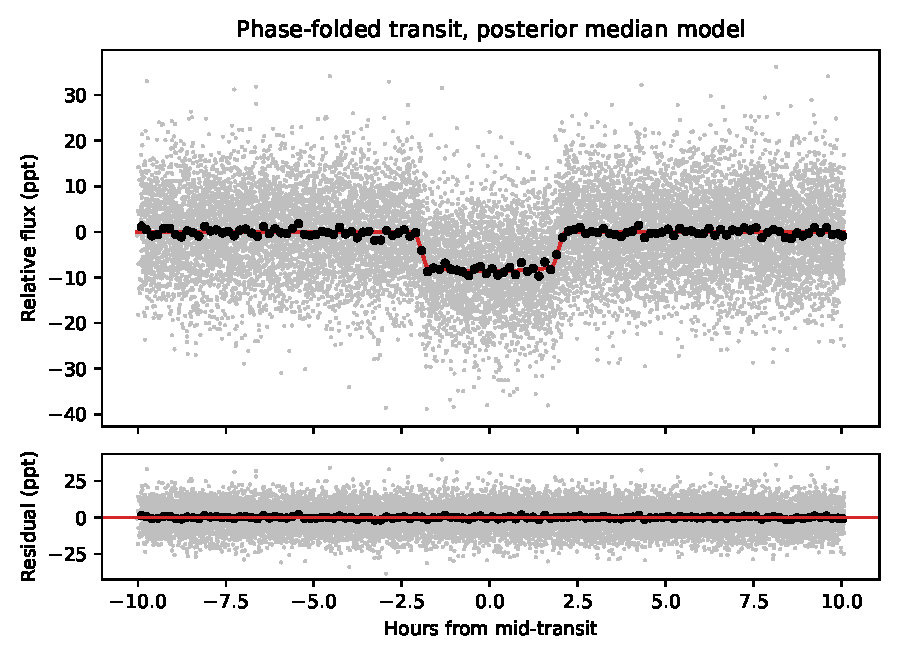
\includegraphics[width=.49\textwidth]{figures/folded_452464529.pdf}
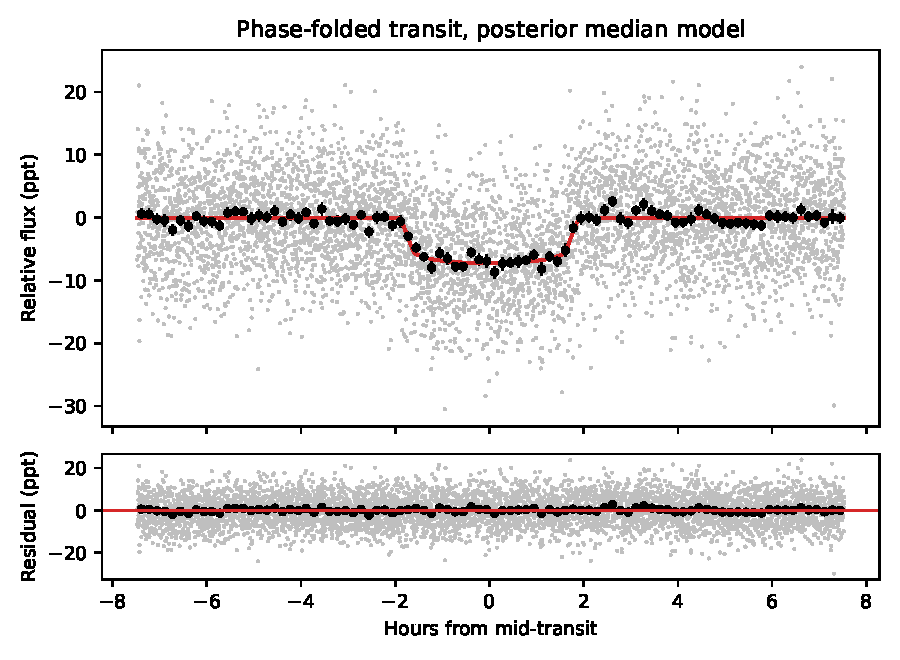
\includegraphics[width=.49\textwidth]{figures/folded_89062142.pdf}
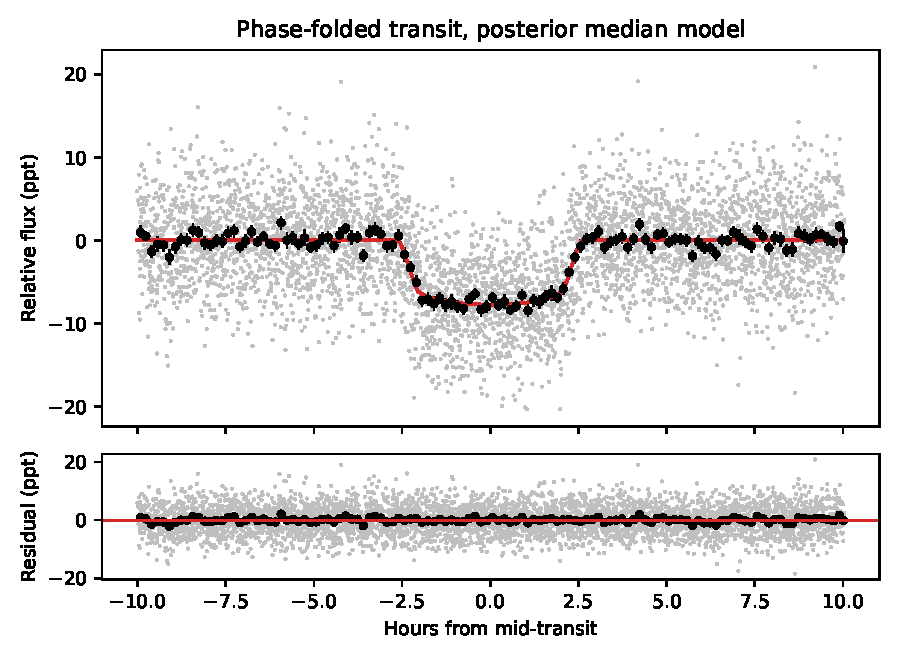
\includegraphics[width=.49\textwidth]{figures/folded_410056850.pdf}
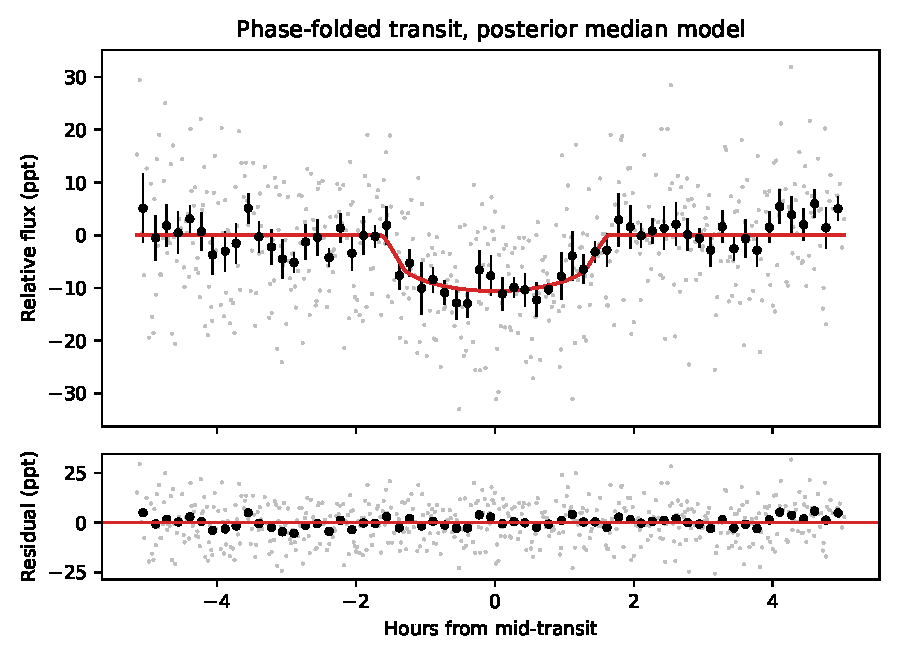
\includegraphics[width=.49\textwidth]{figures/folded_219396153.pdf}
\caption{Phase-folded transits of TOI-3025.01, TOI-4674.01, TOI-7850.01 and TOI-7888.01 (top left
to bottom right) with the posterior median model; black points are 10-minute bins.}
\label{fig:folded}
\end{figure*}

\begin{figure*}
\centering
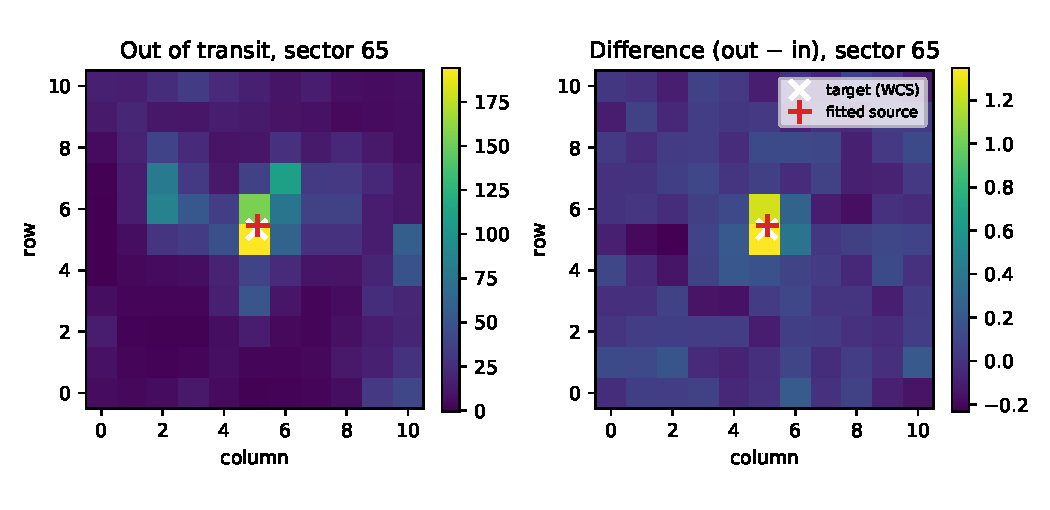
\includegraphics[width=.49\textwidth]{figures/difference_452464529.pdf}
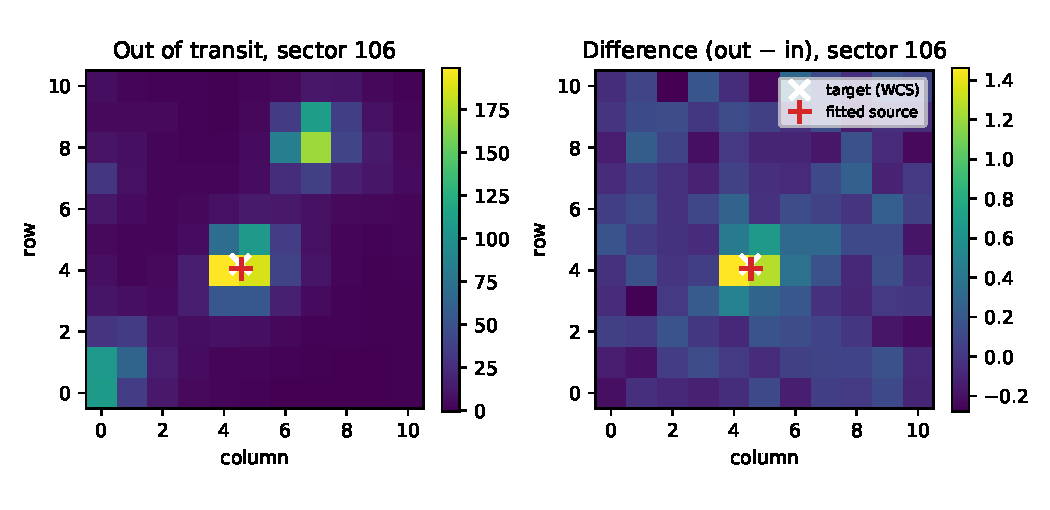
\includegraphics[width=.49\textwidth]{figures/difference_89062142.pdf}
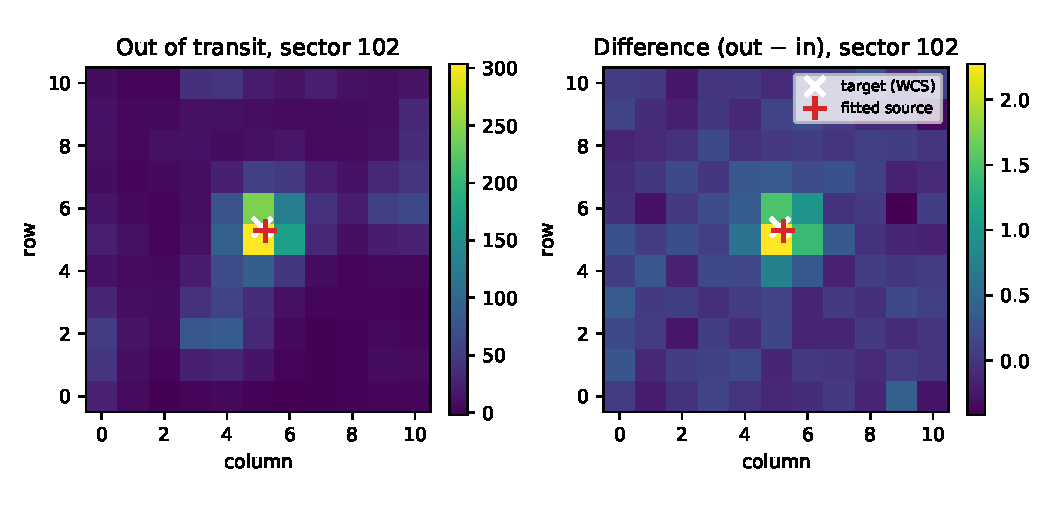
\includegraphics[width=.49\textwidth]{figures/difference_410056850.pdf}
\caption{Out-of-transit and difference images of TOI-3025.01, TOI-4674.01 and TOI-7850.01 in one
sector each (the difference image of TOI-7888.01 is not significant). White crosses
mark the catalogue position of the target; red plus signs the fitted source of the transit signal.}
\label{fig:diff}
\end{figure*}

\clearpage
\subsection{Supplementary tests of initially inconclusive TOIs}\label{sec:inconclusive}
A total of 91 recovered TOIs passed the photometric vetting and were initially classified as inconclusive.
Of these, 86 score below the classifier threshold (raw scores
0.02--0.876, threshold 0.877).
The other 5 (marked with $\dagger$ in Table~\ref{tab:inconclusive}) are selected by the classifier,
but the search \texttt{TRICERATOPS} result falls outside the candidate criterion
(FPP\,$\geq 50\%$, or $0.1\% \leq$\,NFPP\,$\leq 10\%$).
Difference images and \texttt{TRICERATOPS} (three runs) were computed for all of them. None has FPP\,$<1\%$ and NFPP\,$<0.1\%$,
while 17 have FPP\,$<50\%$ and NFPP\,$<0.1\%$, 49 have NFPP\,$>10\%$ (signal likely from a
neighbour), and 2 show a significant difference-image offset ($>4\sigma$ and $>0.5$ pixel).
Signals above the NFPP or offset limits would be rejected by these tests; they are kept in the
table to show the full group.


\startlongtable
\begin{deluxetable*}{lcccccccccc}
\tablecaption{Initially inconclusive recovered TOIs: supplementary source tests and false-positive probabilities.\label{tab:inconclusive}}
\tablehead{\colhead{TOI} & \colhead{TIC} & \colhead{$P$ (d)} & \colhead{Depth (ppm)} & \colhead{SNR} &
\colhead{$R_p$ ($R_\oplus$)} & \colhead{CNN} & \colhead{FPP} & \colhead{NFPP} & \colhead{Offset ($''$)} & \colhead{Offset ($\sigma$)}}
\startdata
TOI-2542.01 & 431971818 & 4.1099 & 33243 & 13.4 & -- & 0.46 & 0.923 & 0.62 & -- & -- \\
TOI-2861.01 & 157572174 & 6.6301 & 5685 & 14.1 & 12.3 & 0.46 & 0.132 & 0.023 & 3.2 & 0.9 \\
TOI-2897.01$^\dagger$ & 308987429 & 12.0041 & 10994 & 40.8 & 11.2 & 0.92 & 1.000 & $1\times 10^{-4}$ & 0.7 & 0.1 \\
TOI-2926.01 & 34499178 & 2.4249 & 7235 & 18.1 & 17.8 & 0.74 & 0.063 & 0.013 & 3.8 & 2.0 \\
TOI-2993.01 & 48768158 & 2.3372 & 5934 & 18.2 & -- & 0.85 & 0.800 & $0$ & 1.5 & 0.4 \\
TOI-3012.01 & 437560683 & 3.0919 & 61168 & 29.8 & -- & 0.46 & 0.875 & 0.38 & 0.4 & 0.1 \\
TOI-3014.01 & 383806208 & 1.7947 & 3859 & 25.2 & 11.4 & 0.18 & 1.000 & 0.98 & 0.5 & 0.1 \\
TOI-3021.01 & 45054849 & 11.2598 & 17883 & 30.9 & -- & 0.85 & 0.889 & 0.44 & 0.5 & 0.1 \\
TOI-3034.01 & 391645374 & 1.4033 & 18905 & 40.4 & -- & 0.05 & 0.967 & 0.83 & -- & -- \\
TOI-3043.01 & 360706000 & 2.3726 & 6797 & 24.2 & 18.7 & 0.18 & 0.994 & 0.6 & 1.2 & 0.4 \\
TOI-3062.01 & 463343283 & 4.8650 & 10389 & 15.4 & 13.5 & 0.40 & 0.994 & 0.98 & 6.1 & 3.2 \\
TOI-3074.01 & 447976172 & 5.3583 & 9486 & 26.6 & -- & 0.85 & 0.933 & 0.67 & 3.6 & 1.4 \\
TOI-3079.01 & 441444262 & 1.9898 & 20273 & 64.4 & -- & 0.46 & 0.938 & 0.69 & 1.1 & 0.4 \\
TOI-3081.01 & 432467894 & 3.4364 & 6942 & 23.2 & 23.9 & 0.68 & 1.000 & 0.045 & 0.9 & 0.2 \\
TOI-3090.01 & 309913305 & 6.3273 & 9067 & 10.3 & -- & 0.66 & 0.957 & 0.78 & 8.5 & 4.8 \\
TOI-3143.01 & 384244834 & 2.9903 & 20475 & 37.5 & -- & 0.18 & 0.996 & 0.97 & 3.2 & 2.0 \\
TOI-3172.01 & 398502253 & 3.0041 & 6468 & 11.9 & 16.8 & 0.42 & 0.529 & 0.29 & 2.7 & 0.9 \\
TOI-3208.01 & 319949055 & 2.3577 & 12193 & 13.4 & 16.8 & 0.42 & 0.065 & $5\times 10^{-4}$ & 1.4 & 0.4 \\
TOI-3209.01 & 319806044 & 1.3509 & 9002 & 9.4 & -- & 0.35 & 1.000 & 0.99 & 2.0 & 0.6 \\
TOI-3258.01 & 369789627 & 1.2280 & 2695 & 20.7 & -- & 0.46 & 0.929 & 0.64 & 5.7 & 3.1 \\
TOI-3307.01 & 369861728 & 3.8781 & 9744 & 21.6 & 12.3 & 0.42 & 0.495 & 0.4 & -- & -- \\
TOI-3387.01 & 118072143 & 2.7678 & 10350 & 22.0 & -- & 0.18 & 0.923 & 0.62 & 1.8 & 0.7 \\
TOI-3393.01 & 173260345 & 5.2060 & 12316 & 19.0 & 13.7 & 0.68 & 0.546 & 0.34 & 1.4 & 0.5 \\
TOI-3421.01 & 145023816 & 2.8389 & 6912 & 19.3 & 19.4 & 0.35 & 0.458 & 0.08 & 0.9 & 0.1 \\
TOI-3425.01 & 144682439 & 0.7654 & 3300 & 12.0 & 9.5 & 0.29 & 0.974 & 0.78 & -- & -- \\
TOI-3439.01 & 394338713 & 5.9350 & 13543 & 32.1 & 14.4 & 0.18 & 0.979 & 0.56 & 1.9 & 0.8 \\
TOI-3463.01 & 292889298 & 2.2532 & 19798 & 17.2 & -- & 0.75 & 0.944 & 0.72 & -- & -- \\
TOI-4169.01 & 372747949 & 3.4027 & 3766 & 45.8 & 14.6 & 0.75 & 0.278 & $2\times 10^{-6}$ & 1.7 & 0.6 \\
TOI-4228.01 & 415143674 & 6.0167 & 13460 & 19.1 & 20.1 & 0.46 & 0.354 & 0.13 & 1.3 & 0.2 \\
TOI-4720.01 & 124322274 & 3.7814 & 11474 & 12.2 & 18.5 & 0.46 & 0.356 & 0.015 & 0.4 & 0.0 \\
TOI-4793.01 & 65949719 & 3.4629 & 11027 & 24.9 & 17.1 & 0.68 & 0.177 & $8\times 10^{-5}$ & 1.0 & 0.1 \\
TOI-4796.01 & 65905621 & 3.5776 & 10545 & 27.9 & 18.1 & 0.42 & 0.716 & 0.36 & 1.0 & 0.2 \\
TOI-4802.01 & 50575306 & 1.7167 & 8496 & 15.2 & 10.9 & 0.08 & 0.995 & 0.99 & 12.8 & 5.0 \\
TOI-4815.01 & 19447218 & 8.9727 & 10405 & 11.1 & 13.5 & 0.74 & 0.484 & 0.3 & 4.4 & 1.2 \\
TOI-4870.01 & 446135868 & 1.8119 & 7871 & 19.7 & 9.3 & 0.35 & 0.992 & 0.98 & 5.6 & 2.9 \\
TOI-4874.01 & 463754499 & 2.2867 & 4967 & 11.3 & 18.6 & 0.35 & 0.866 & 0.47 & 8.0 & 2.4 \\
TOI-4881.01 & 359735804 & 4.4159 & 8141 & 28.7 & 19.9 & 0.68 & 0.238 & $4\times 10^{-4}$ & 0.2 & 0.0 \\
TOI-4884.01 & 80681136 & 1.5305 & 5133 & 18.3 & -- & 0.42 & 0.941 & 0.71 & 1.6 & 0.3 \\
TOI-4894.01 & 469333534 & 3.5611 & 7434 & 8.8 & -- & 0.42 & 0.957 & 0.78 & 10.2 & 3.9 \\
TOI-4900.01 & 425508314 & 7.6650 & 8481 & 28.2 & 16.9 & 0.85 & 0.602 & $5\times 10^{-11}$ & -- & -- \\
TOI-4910.01 & 303327435 & 5.5075 & 16331 & 15.8 & 14.1 & 0.50 & 0.785 & 0.3 & -- & -- \\
TOI-4924.01 & 307099276 & 3.1468 & 14486 & 18.4 & -- & 0.35 & 0.994 & 0.83 & 1.5 & 0.2 \\
TOI-4943.01 & 418567812 & 8.0176 & 19106 & 21.9 & -- & 0.85 & 0.329 & 0.31 & 0.4 & 0.1 \\
TOI-4975.01 & 304085024 & 4.4835 & 7228 & 19.8 & -- & 0.19 & 0.999 & 0.87 & -- & -- \\
TOI-5033.01$^\dagger$ & 318180448 & 5.4696 & 1506 & 12.2 & 1.5 & 0.96 & 0.090 & $4\times 10^{-3}$ & -- & -- \\
TOI-5039.01 & 396649769 & 2.1968 & 5442 & 8.1 & 14.5 & 0.66 & 0.506 & 0.037 & 3.4 & 1.1 \\
TOI-5046.01 & 306512967 & 11.1837 & 5939 & 17.5 & -- & 0.75 & 0.206 & 0.18 & -- & -- \\
TOI-5064.01 & 407127579 & 3.5108 & 1223 & 16.7 & 6.1 & 0.66 & 0.273 & 0.23 & -- & -- \\
TOI-5922.01 & 364192929 & 5.2054 & 11149 & 17.6 & 20.6 & 0.66 & 0.818 & $0$ & 4.4 & 1.0 \\
TOI-6259.01 & 294497466 & 3.2387 & 559 & 7.1 & 5.6 & 0.05 & 0.810 & 0.22 & -- & -- \\
TOI-6453.01 & 66242670 & 6.8669 & 5412 & 16.8 & 15.9 & 0.42 & 0.403 & 0.37 & 10.0 & 2.8 \\
TOI-6464.01 & 190643105 & 9.6741 & 3653 & 23.6 & 17.5 & 0.68 & 0.014 & $6\times 10^{-6}$ & 3.7 & 0.9 \\
TOI-6471.01 & 410901394 & 3.0761 & 2399 & 10.8 & 6.1 & 0.66 & 0.485 & 0.43 & -- & -- \\
TOI-6472.01 & 140706833 & 2.6819 & 6294 & 20.8 & 17.3 & 0.42 & 0.270 & 0.26 & 2.6 & 0.8 \\
TOI-6477.01 & 11927677 & 3.6861 & 7626 & 46.3 & 16.8 & 0.42 & 0.221 & 0.02 & 2.1 & 0.5 \\
TOI-6485.01 & 281286325 & 17.0184 & 14804 & 32.0 & 16.7 & 0.89 & 0.456 & $0$ & 2.9 & 1.3 \\
TOI-6487.01 & 37754672 & 7.0678 & 3754 & 19.8 & 10.3 & 0.42 & 0.659 & 0.017 & 2.3 & 0.6 \\
TOI-6490.01 & 118754987 & 7.8420 & 7118 & 19.9 & 14.1 & 0.75 & 0.062 & $6\times 10^{-7}$ & 5.3 & 1.0 \\
TOI-6504.01 & 177257073 & 6.8327 & 5072 & 25.3 & 11.3 & 0.75 & 0.792 & 0.78 & 1.1 & 0.1 \\
TOI-6536.01 & 280647591 & 4.2379 & 6311 & 13.8 & 8.5 & 0.75 & 0.953 & 0.94 & 0.2 & 0.0 \\
TOI-6537.01 & 80384677 & 3.6480 & 3001 & 10.6 & -- & 0.74 & 0.787 & 0.75 & -- & -- \\
TOI-6544.01 & 161738745 & 3.6250 & 874 & 18.2 & -- & 0.85 & 0.933 & 0.67 & -- & -- \\
TOI-6545.01 & 72504017 & 5.6178 & 450 & 8.9 & 5.7 & 0.18 & 0.598 & 0.056 & -- & -- \\
TOI-6554.01 & 94483093 & 5.2309 & 1100 & 12.6 & 5.3 & 0.46 & 0.209 & 0.16 & -- & -- \\
TOI-6555.01 & 259606227 & 10.1286 & 526 & 12.9 & 4.7 & 0.85 & 0.009 & $2\times 10^{-3}$ & -- & -- \\
TOI-6558.01 & 420529106 & 9.5307 & 1399 & 14.9 & 2.9 & 0.45 & 0.019 & $4\times 10^{-3}$ & -- & -- \\
TOI-6565.01 & 392914193 & 0.8775 & 1960 & 21.7 & 7.1 & 0.42 & 0.482 & $9\times 10^{-13}$ & 2.6 & 0.5 \\
TOI-6590.01 & 72123144 & 7.0838 & 8442 & 9.2 & 13.7 & 0.43 & 0.543 & 0.48 & 6.2 & 1.3 \\
TOI-6591.01 & 463868678 & 5.7831 & 1504 & 12.1 & 15.8 & 0.42 & 0.291 & $7\times 10^{-4}$ & -- & -- \\
TOI-6595.01 & 361344753 & 7.5157 & 1454 & 13.7 & 3.7 & 0.89 & 0.079 & 0.05 & -- & -- \\
TOI-6827.01 & 302453291 & 4.4642 & 2690 & 14.4 & 14.3 & 0.85 & 0.472 & $2\times 10^{-4}$ & -- & -- \\
TOI-7465.01 & 167804011 & 6.2057 & 4552 & 19.7 & 8.7 & 0.89 & 0.012 & $0$ & 3.3 & 0.7 \\
TOI-7488.01 & 128168083 & 3.9050 & 19046 & 17.4 & 17.6 & 0.85 & 0.539 & $1\times 10^{-3}$ & 4.1 & 0.9 \\
TOI-7602.01 & 156716001 & 10.3048 & 656 & 8.0 & 3.0 & 0.86 & 0.017 & 0.0074 & -- & -- \\
TOI-7639.01$^\dagger$ & 270471727 & 10.4564 & 662 & 11.7 & 2.8 & 0.92 & 0.009 & $1\times 10^{-3}$ & -- & -- \\
TOI-7682.01 & 159671133 & 1.3438 & 168 & 8.4 & 2.8 & 0.18 & 0.619 & 0.51 & -- & -- \\
TOI-7684.01 & 115942852 & 3.2112 & 7992 & 9.0 & 6.6 & 0.86 & 0.359 & 0.3 & 0.1 & 0.0 \\
TOI-7686.01 & 273861354 & 13.9967 & 15774 & 13.2 & 9.2 & 0.86 & 0.392 & 0.06 & 3.1 & 0.4 \\
TOI-7689.01 & 12999193 & 1.4830 & 20865 & 25.3 & 4.0 & 0.85 & 0.954 & $0$ & 5.5 & 1.9 \\
TOI-7701.01 & 122522333 & 20.6077 & 2053 & 29.8 & 8.7 & 0.85 & 0.038 & $8\times 10^{-6}$ & 92.7 & 8.0 \\
TOI-7705.01 & 70514245 & 4.0478 & 20686 & 80.0 & 12.6 & 0.86 & 0.306 & $3\times 10^{-4}$ & 0.7 & 0.2 \\
TOI-7711.01 & 1309019 & 3.2423 & 9027 & 19.4 & 13.8 & 0.46 & 0.109 & 0.0098 & 3.4 & 0.9 \\
TOI-7712.01 & 264460009 & 3.0934 & 22301 & 25.1 & 15.3 & 0.46 & 0.902 & 0.85 & 0.6 & 0.0 \\
TOI-7713.01 & 77287067 & 4.0763 & 14294 & 30.0 & 16.9 & 0.85 & 0.052 & $4\times 10^{-5}$ & 1.5 & 0.4 \\
TOI-7720.01 & 421184129 & 8.0315 & 1807 & 13.8 & 14.7 & 0.18 & 0.283 & $3\times 10^{-7}$ & -- & -- \\
TOI-7723.01$^\dagger$ & 162093661 & 6.3338 & 5631 & 7.3 & 4.6 & 0.92 & 0.039 & 0.02 & -- & -- \\
TOI-7762.01 & 193318850 & 7.8592 & 4920 & 12.7 & 6.1 & 0.89 & 0.102 & $0$ & -- & -- \\
TOI-7822.01 & 146320244 & 4.4938 & 1820 & 11.9 & 5.0 & 0.75 & 0.257 & 0.2 & -- & -- \\
TOI-7824.01$^\dagger$ & 73644471 & 4.5966 & 9726 & 36.7 & 15.4 & 0.93 & 0.586 & $0$ & 6.2 & 1.9 \\
TOI-7825.01 & 193096383 & 4.8565 & 3531 & 18.2 & 6.3 & 0.74 & 0.043 & $0$ & 1.3 & 0.1 \\
TOI-7854.01 & 124095894 & 1.1257 & 9926 & 12.0 & -- & 0.42 & 0.909 & 0.55 & -- & -- \\
\enddata
\tablecomments{Depth, SNR and radius from the box model of the vetting; FPP and NFPP from three
TRICERATOPS runs; offset of the difference-image source from the target. Dashes: not computed or
image not significant. Membership in this table follows the initial search tier; supplementary rejection criteria are discussed in the text.}
\end{deluxetable*}


The supplementary tests separate a few cases. TOI-4802.01 ($P=1.72$\,d) is most likely a nearby
eclipsing binary: the difference-image source lies $12.8''$ from the target at $5\sigma$ and
NFPP\,$=0.99$. TOI-7701.01 ($P=20.6$\,d) has a low FPP (0.04), but its only significant difference
image (one transit, sector~106) places the source $93''$ (4.4 pixels) from the target at $8\sigma$; the
FPP does not account for this, and the signal should be treated as a possible blend until more transits
are imaged. Both fail the pixel test. Among the signals located on the target, TOI-7465.01, TOI-6464.01, TOI-7825.01 and TOI-7713.01 have
FPP\,$\approx 1$--$5\%$ and NFPP\,$<0.01\%$ from three runs.
TOI-7465.01, with FPP\,$=1.2\%$, has a raw classifier score of 0.856, just below the 0.877
threshold. These four are worth following up even though the classifier did not select them.

\subsection{Signals not in any catalogue}
A total of 15 signals in these stars pass the photometric vetting but match no catalogued signal
(Table~\ref{tab:new}). None is selected by the classifier. Each lies in the host star of an open
TOI and does not coincide with it in period or phase; they are listed with the same supplementary
tests as a starting point for inspection, not as planet candidates.


\startlongtable
\setlength{\tabcolsep}{3.5pt}
\begin{deluxetable*}{lcccccccccccc}
\tabletypesize{\scriptsize}
\tablecaption{Signals that pass the photometric vetting and match no catalogued signal.\label{tab:new}}
\tablehead{\colhead{TIC} & \colhead{Host TOI} & \colhead{$P$ (d)} & \colhead{$T_0-2460000$} & \colhead{$T_{14}$ (h)} &
\colhead{Depth (ppm)} & \colhead{SNR} & \colhead{$N_{\rm tr}$} & \colhead{$R_p$ ($R_\oplus$)} & \colhead{CNN} &
\colhead{FPP} & \colhead{NFPP} & \colhead{Offset ($''$)}}
\startdata
66620917 & TOI-4391.01 & 0.6166 & 69.3666 & 0.75 & 1470 & 15.8 & 102 & -- & 0.42 & 1.000 & $8\times 10^{-8}$ & 17.1 \\
81089255 & TOI-6480.01 & 66.5924 & -744.7652 & 1.50 & 2571 & 8.2 & 2 & 7.9 & 0.40 & 0.880 & 0.26 & 93.6 \\
105712339 & TOI-7754.01 & 22.9961 & 1067.4995 & 1.50 & 6892 & 14.2 & 2 & 10.1 & 0.18 & 0.786 & 0.096 & -- \\
255560319 & TOI-6703.01 & 92.6536 & -1605.7942 & 1.50 & 448 & 7.4 & 3 & 5.7 & 0.35 & 1.000 & $0$ & -- \\
259606227 & TOI-6555.01 & 1.0644 & 1046.5423 & 2.50 & 185 & 12.1 & 60 & 2.8 & 0.08 & 0.066 & 0.061 & -- \\
261746870 & TOI-7710.01 & 72.0614 & -1658.7563 & 0.50 & 2550 & 12.6 & 2 & 5.0 & 0.46 & 0.999 & $0$ & -- \\
292889298 & TOI-3463.01 & 0.5014 & 69.0558 & 1.00 & 9246 & 8.8 & 102 & -- & 0.35 & 0.973 & 0.86 & -- \\
294497466 & TOI-6259.01 & 0.6550 & 718.6830 & 2.00 & 267 & 7.8 & 79 & 3.9 & 0.01 & 0.134 & 0.12 & -- \\
303327435 & TOI-4910.01 & 61.1731 & 34.0786 & 10.00 & 14113 & 9.6 & 3 & 13.1 & 0.42 & 0.603 & 0.52 & -- \\
306512967 & TOI-5046.01 & 0.7532 & -35.2373 & 2.50 & 481 & 7.3 & 479 & -- & 0.04 & 0.342 & 0.33 & -- \\
369861728 & TOI-3307.01 & 13.0871 & 69.6090 & 6.00 & 3324 & 8.5 & 3 & 7.2 & 0.46 & 0.628 & 0.62 & -- \\
391645374 & TOI-3034.01 & 1.4908 & 15.6886 & 2.50 & 3165 & 7.6 & 40 & -- & 0.19 & 0.989 & 0.95 & -- \\
407827885 & TOI-4963.01 & 41.7279 & 99.4532 & 0.75 & 14298 & 7.7 & 2 & -- & 0.85 & 0.955 & 0.77 & -- \\
420529106 & TOI-6558.01 & 21.9609 & 1049.7166 & 3.00 & 954 & 9.6 & 4 & 2.4 & 0.85 & 0.034 & 0.013 & -- \\
425508314 & TOI-4900.01 & 13.0538 & 54.8459 & 1.50 & 4741 & 10.2 & 4 & 12.6 & 0.35 & 0.791 & 0.095 & -- \\
\enddata
\tablecomments{Box-model parameters from the vetting; $T_0$ in BJD$_{\rm TDB}$. FPP, NFPP and difference-image offset from
the supplementary analysis (three TRICERATOPS runs).}
\end{deluxetable*}


Two of these signals are off target: the difference images of TIC~66620917 ($P=0.62$\,d) and
TIC~81089255 ($P=66.6$\,d) place the source $17''$ ($12\sigma$) and $94''$ ($26\sigma$) from the
target, so both are attributed to neighbouring stars. The most promising is TIC~420529106
($P=21.96$\,d, four transits, depth 954\,ppm, $R_p\approx2.4\,R_\oplus$, SNR 9.6), with a
calibrated score of 0.85, FPP\,$=0.03$ and NFPP\,$=0.01$; its difference image is not significant.
TIC~259606227 ($P=1.06$\,d, $R_p\approx2.8\,R_\oplus$) has FPP\,$=0.07$ but a classifier score of
0.08. At SNR near 10, both need more data before they can be considered candidates.

\section{Discussion}\label{sec:discussion}

\textit{Classifier domain.} The network is trained on labelled TOIs, and its precision
applies to that population. On 200 inverted single-sector light curves
the full pipeline selected one noise signal, but the classifier was designed for high precision and
selects about half of the confirmed planets; a classifier score below threshold is weak evidence
against a planet.

\textit{False-positive probabilities.} The FPPs are computed without high-resolution imaging, so
close bound companions are only constrained by the TIC and Gaia. The Monte Carlo scatter of
\texttt{TRICERATOPS} is comparable to the differences between some candidates, which is why the
candidate values average ten runs; the quoted errors cover only this scatter, not the priors. An
NFPP of zero means that no simulated nearby scenario reproduced the transit, not that contamination
is excluded. None of our signals is statistically validated.

\textit{Completeness.} The sample is restricted to stars with 120\,s data. The periodic search covers
0.5--100\,d, and the isolated-event search has limited sensitivity to longer periods.
TOIs detected in sectors without 120\,s data may be missed. The recovery fraction of catalogued
TOIs is not a population completeness, and the injection tests use trapezoidal signals.

\textit{Follow-up.} The candidates are suitable for reconnaissance spectroscopy, which would identify
eclipsing binaries through radial-velocity variations of kilometres per second, and for
high-resolution imaging, which would constrain close companions and inform revised FPPs.

\section{Conclusions}\label{sec:conclusions}
A pipeline that combines a blind periodic and long-period search, photometric, centroid,
systematic and pixel-level tests, a cross-validated neural network and \texttt{TRICERATOPS} recovers
\nRecovered{} of the \nOpen{} open TOIs with 120\,s data. Four of them
meet our candidate-selection criteria, three have difference images consistent with the target
position, and their FPPs
are 1.7--34\%. We list the
results for every recovered TOI and the uncatalogued signals that pass the photometric vetting, as a
prioritization aid for follow-up observations: after the four candidates, the on-target TOIs
TOI-7465.01, TOI-6464.01, TOI-7825.01 and TOI-7713.01 and the uncatalogued signal of TIC~420529106
are the most promising.

\section*{Data and code availability}
The TESS observations used in this work are available from MAST; the TOI catalogue and follow-up
records were retrieved from ExoFOP as described in Section~\ref{sec:data}.
The analysis code and results are available at
\url{https://github.com/nrolabs/tess-open-tois}.

\begin{acknowledgments}
This paper includes data collected by the TESS mission, funded by the NASA Science Mission
Directorate, obtained from MAST at the Space Telescope Science Institute. This research has made use
of the Exoplanet Follow-up Observation Program website and the NASA Exoplanet Archive, operated by
the California Institute of Technology under contract with NASA.
\end{acknowledgments}

\facilities{TESS, MAST, ExoFOP}

\software{astropy \citep{Astropy2022}, batman \citep{Kreidberg2015}, emcee \citep{ForemanMackey2013},
lightkurve \citep{Lightkurve2018}, numpy \citep{Harris2020}, PyTorch \citep{Paszke2019},
scikit-learn \citep{Pedregosa2011}, scipy \citep{Virtanen2020}, TRICERATOPS \citep{Giacalone2021},
pytransit \citep{Parviainen2015}}

\bibliographystyle{aasjournalv7}
\bibliography{references}

\end{document}
